\begin{post}
	\postdata{The best city tour ever and the tower of love}{2011}{9}{17}{1}{20}{17}
	\begin{content}
City tour. We have all been there. Unknown city or place, a bus full of people, boring commentary (stupid jokes included). Well, since we are not only students, but also tourists here, we have decided to give it a go. Well, Karin has decided and few of us joined her. We had nothing to do anyway, since it was Chuseok Monday and most places were closed. The plan was to take the night tour, which is a 1:30h bus tour through the Seoul city center, including the N Seoul Tower. And the plan failed big time. Now we know that it can take more than a hour to get from our campus to the Gwanghwamun station. Yes, despite our heroic effort and a subway transfer sprint, we missed the bus. Well, both of them, actually — OK, Time For Plan B. We have decided to roam around the neighborhood, look at the statue of King Sejong and other things. And it was really nice.

%\begin{figure}[h]
%\centering
%\subfigure[Gwanghwamun station neighborhood]{\fbox{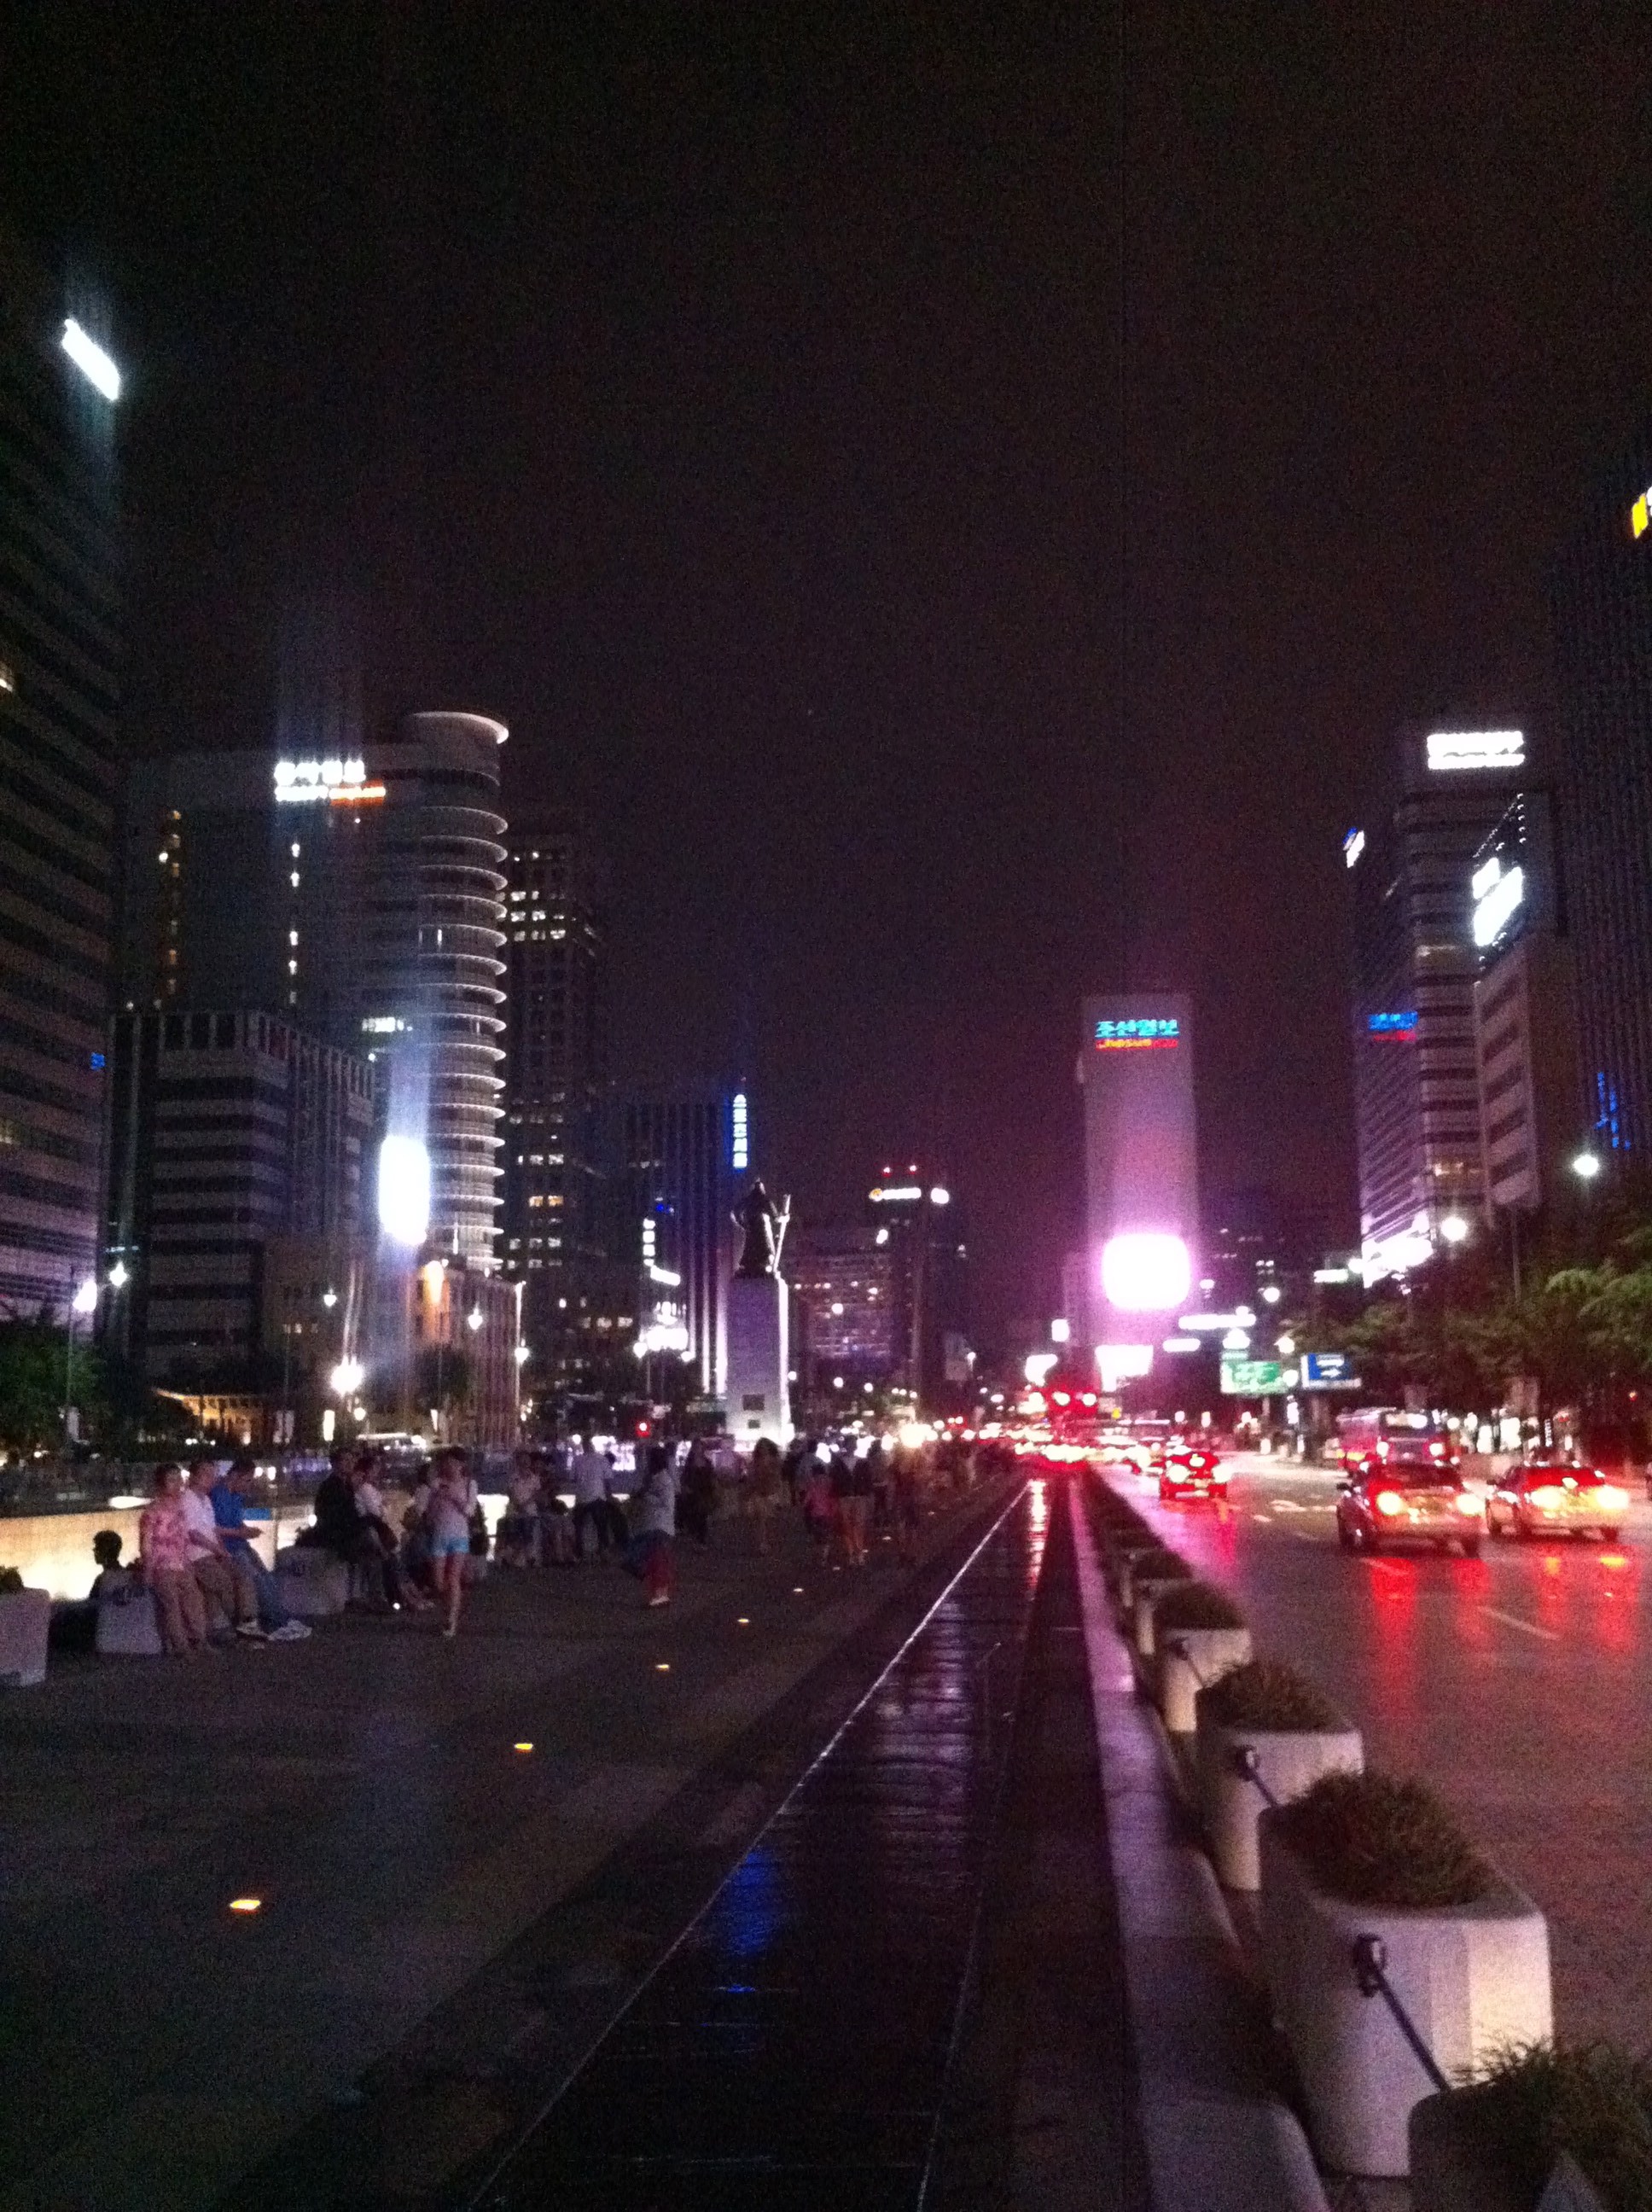
\includegraphics[width=0.32\textwidth]{photos/09/17/img_1141.jpg}}}
%\subfigure[Chuesok celebration]{\fbox{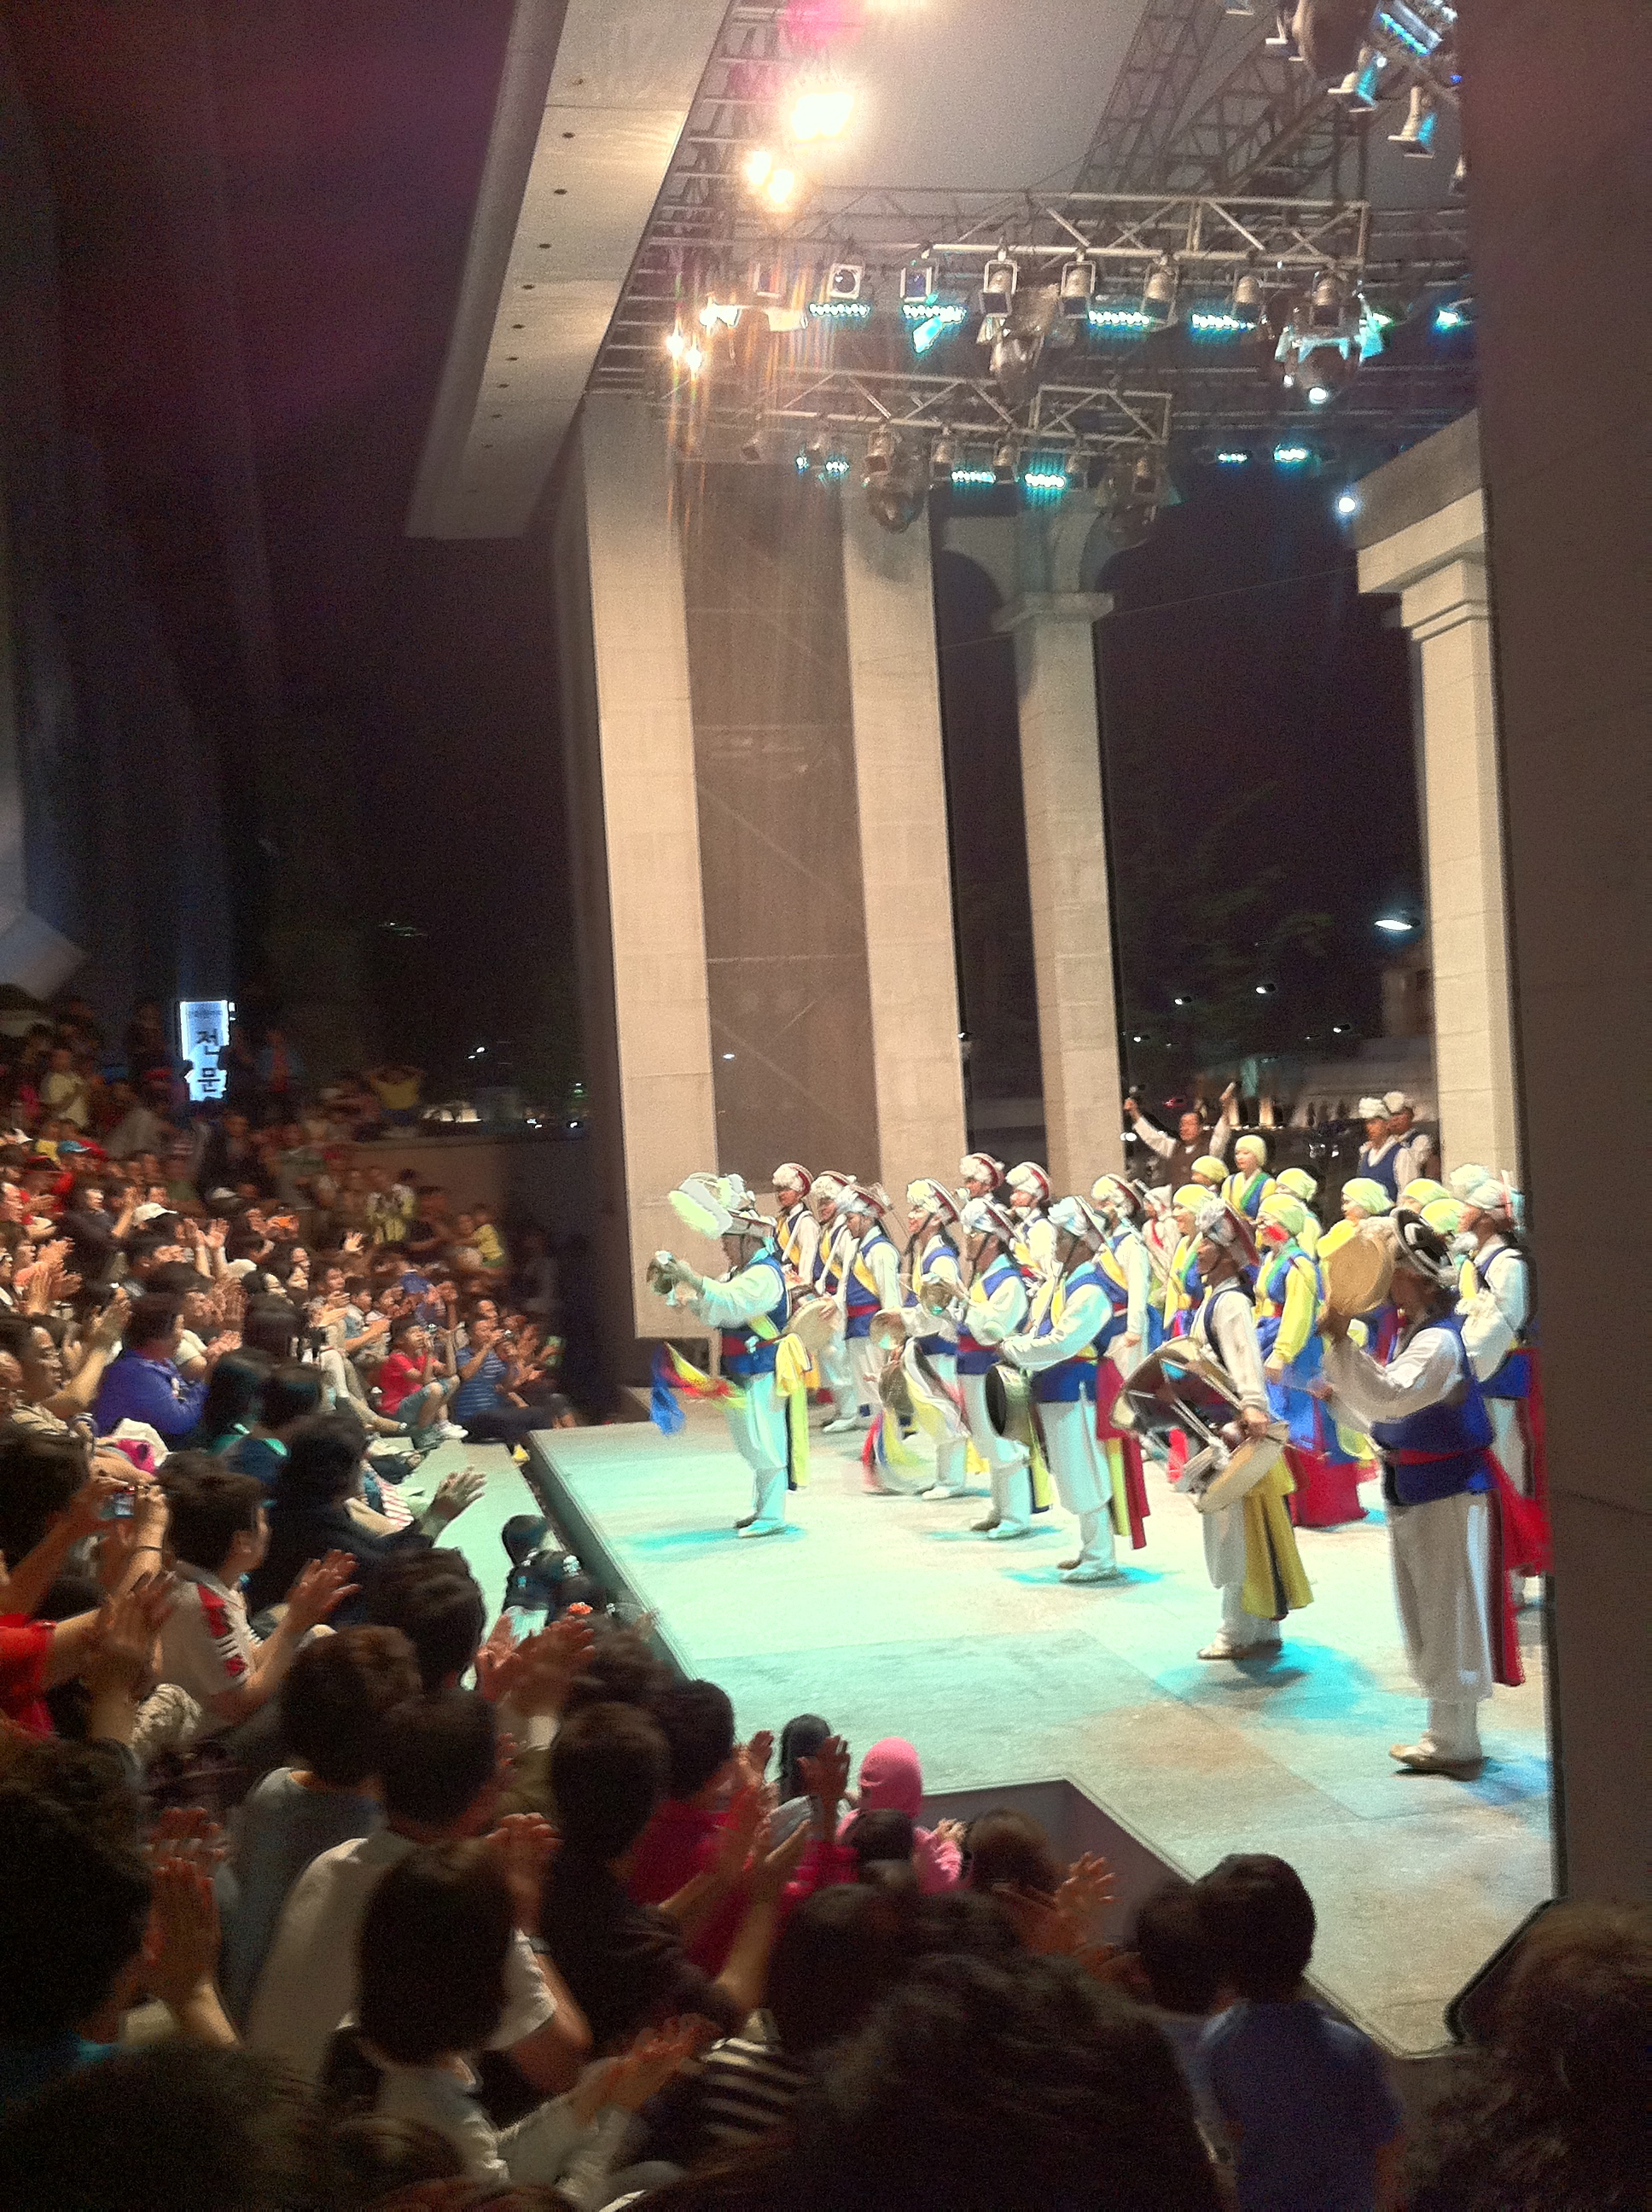
\includegraphics[width=0.32\textwidth]{photos/09/17/img_1154.jpg}}}
%\end{figure}

We saw a Chuseok celebration with some acrobats/dancers, which was awesome. Since we were quite close to the "cozy part of Seoul", which we discovered after our "hiking" trip, we decided to go there and try find some nice place to get food and drinks. That proved to be quite difficult, because nearly all places were either closed because of Chuseok or were closing because it was already around 9:30pm. Eventually we found a nice place, where we got delicious dumplings. Huge and delicious. They are filled with minced meat and some veggies, and fill you up immediately. And they are not that spicy!

Tuesday was more exciting. Not only the shops and restaurants were open again, but we also decided to go to the N Seoul Tower, which is, for unknown reasons, portrayed as a love tower. Supposedly, the Namsan Mountain, where the tower is located is some kind of a "first love" place. Some say, that you should go there with your first love and put a lock with some personal message on the fence there. The fence is just packed with locks, and they even have to take some away every year, otherwise the whole thing would be too heavy and there would not be any place for another firstlovers.

%[caption id="" align="aligncenter" width="375" caption="N Seoul Tower — via flickr"]<img title="N Seoul Tower" src="http://farm2.static.flickr.com/1306/851500946_e1abf7512e.jpg" alt="" width="375" height="500" />[/caption]

I was quite surprised by the number of people around the tower. I honestly expected that it would be nearly deserted place, but the park around the tower was packed with people, mostly Koreans. Seems like Namsan is a favorite place to hang out in Seoul. Anyway, the view was terrific and we even managed to locate our campus. Or at least the black spot where the campus was supposed to be. Guess we should have told someone to light a bonfire at the roof for better identification.

Anyway, sometimes it is nice to be a tourist, especially when you know the place a little. There are still thousands of places in Seoul that are worth visiting, from the Dongdaemun market to the War Museum. We also want to visit the DMZ and some other places in Korea, of course. But we'll see, school is getting more and more intensive and even though this is an exchange, one has to work as well.

%N.B.: Photos shamelessly stolen from <a href="http://seoulong.wordpress.com">Karin</a>. Thanks!:)
	\end{content}
\end{post}
